\section{CLOS}
Grundlage für dieses Kapitel ist das Buch ``Object-Oriented Programming in Common Lisp. A Programmer's Guide to CLOS'' \cite{keene} von Sonya E. Keene. 

Das Common Lisp Object System ist der Standard für objektorientierte Programmierung in der Sprache Common Lisp. Auch Racket bietet es an, in diesem Stil objektorientiert zu programmieren. Um anstatt des Racketobjektsystems mit CLOS-Objekten zu arbeiten, muss lediglich die Sprache auf den Dialekt Swindle umgestellt werden:


\begin{lstlisting}
#lang swindle
\end{lstlisting}

Es sollen die Klassen Thing, Element, Animal und Pokemon auch in CLOS implementiert werden, um zu sehen, welche Unterschiede in der Syntax es gibt und wie Mehrfachvererbung hier umgesetzt wird. 

Alle Codebeispiele befinden sich auch auf der beiliegenden CD und sind noch einmal zusammenhängend in Anhang \ref{clos-example} aufgeführt.

\subsection{Einfache Klassen}
Für die Definition von Klassen in CLOS gibt es das Makro \texttt{defclass}. Im Gegensatz zu dem Objektsystem von Racket erstellt das Makro eine benannte Klasse. Der Name wird beim Aufruf mit übergeben; damit erübrigt sich eine anschließende Benennung mit \texttt{define}. Auch in CLOS wird die Superklasse mit angegeben. Da es jedoch mehrere Superklassen geben kann, werden diese in einer Liste übergeben. Hat die Klasse keine Superklassen (außer der Wurzelklasse), so wird die leere Liste übergeben. Die explizite Angabe der Wurzelklasse als Superklasse ist nicht nötig. Anschließend können noch die Felder der Klasse (oder Slots, wie sie in CLOS üblicherweise genannt werden) angegeben werden. Für eine minimale Klasse ohne Superklasse(n) genügt der Name und die leere Liste: 

\begin{lstlisting}
(defclass Thing ())
\end{lstlisting}

% Zur Objekterzeugung gibt es in CLOS zwei verschiedene Möglichkeiten, je nachdem ob \texttt{:automaker} als Klassen-Option gesetzt wurde oder nicht. 

Objekte dieser Klasse können mit dem Schlüsselwort \texttt{make} erzeugt werden.

\begin{lstlisting}
> (make Thing)
\end{lstlisting}
{\routput \#Thing}

Slots werden nach der Superklasse angegeben. Ein großer Unterschied zu dem Objektsystem von Racket ist, dass innerhalb einer Klassendefinition \textit{nur} Slots definiert werden, keine Methoden. Methoden werden außerhalb der Klasse definiert. Das bedeutet, dass kein Schlüsselwort notwendig ist, um anzugeben, ob gerade ein Slot oder eine Methode definiert wird. Für die Definition des Namens reicht es zu schreiben:

\begin{lstlisting}
(defclass Thing ()
  (name))
\end{lstlisting}

Die Klasse hat genau einen Slot namens \texttt{name}, der jedoch alleinstehend noch nicht sehr nützlich ist.

Damit mit diesem Slot auch interagiert werden kann, benötigt er noch Accessoren: einen Getter (in CLOS Reader genannt) und einen Setter (in CLOS Writer genannt). Außerdem  ist es gegebenenfalls nötig, einen Initialwert anzugeben, der Slot zu dokumentieren, typisieren und so weiter. All dies geschieht durch Slotoptionen. Sie folgen nach dem Namen des Slots und beginnen per Konvention mit einem Doppelpunkt. Um auf das Attribut \texttt{name} beispielsweise lesend oder schreibend zugreifen zu können, kann die Slotoption \texttt{:reader} beziehungsweise \texttt{:writer} gesetzt werden oder, falls beides über das gleiche Schlüsselwort möglich sein soll, auch die Option \texttt{:accessor}. Accessoren müssen benannt werden, der Name muss sich jedoch nicht vom Namen des Slots unterscheiden. Hier also die vollständige Definition der Klasse:

\begin{lstlisting}
(defclass Thing ()
  (name :accessor name
        :initarg :name
        :initvalue "a Thing")
  :printer #t
  :automaker #t)
\end{lstlisting}

Für die Klasse gibt es drei nützliche Slot- und Klassenoption: \texttt{:initarg}, \texttt{:printer} und \texttt{:automaker}. Die \texttt{:initarg}-Option bewirkt, dass der Parameter bei der Objekterzeugung initialisiert werden kann.

Durch die \texttt{:printer}-Option liefert der Aufruf der \texttt{print}-Funktion an einem Objekt oder die Auswertung des Objekts in der Direkteingabe einen formattierten String. Das hat den Vorteil, dass zur Überprüfung des Zustandes des Objekts nicht jeder Slot einzeln abgefragt werden muss.

\begin{lstlisting}
(make Thing :name "Bob")
\end{lstlisting}
{\routput \#<Thing: name={\qq}Bob\qq>}

\texttt{:automaker} bewirkt, dass es zusätzlich zu dem Schlüsselwort \texttt{make} zur Erzeugung von allgemeinen Objekten mit namensbasierten Initialisierungsargumenten auch das Schlüsselwort \texttt{make-Thing} zur Erzeugung von Objekten der Klasse Thing mit positionsbasierten Parametern gibt. Thing-Objekte können natürlich auch weiterhin mit \texttt{make} erzeugt werden.

\begin{lstlisting}
(make Thing :name "Bob")
(make-Thing "Bob")
\end{lstlisting}

Der Wert eines Slots, der einen Writer oder Accessor besitzt, kann nach der Objekterzeugung mittels \texttt{set!} verändert werden:

\begin{lstlisting}
(define thing (make Thing))
> (set! (name thing) "Bob")
> (name thing)
\end{lstlisting}
{\routput {\qq}Bob\qq}

Eine weitere nützliche Klassenoption ist \texttt{:autoaccessors :slot}, die automatisch für jeden Slot Accessorfunktionen generiert. Der Name der Accessorfunktion ist dann identisch zum Slot. Sie wird für die Klassen Element und Animal verwendet.

\begin{lstlisting}
(defclass Element (Thing)
  (name :initvalue "an Element") 
  (attr :initvalue 'water)
  :autoaccessors :slot 
  :printer #t          
  :automaker #t)
  
(defclass Animal (Thing)
  (name :initvalue "an Animal")      
  (size :initvalue 'small)
  :autoaccessors :slot
  :automaker #t
  :printer #t)
\end{lstlisting}

Der geerbte Slot lässt sich ohne weiteres redefinieren. Da im Folgenden die Objekte nur noch mit \texttt{make-} erzeugt werden, wurde die \texttt{:initarg}-Option weggelassen. Es können beliebig viele Argumente an \texttt{make-} übergeben werden, im Zweifelsfall werden die Slots mit Standardwerten belegt oder überschüssige Parameter ignoriert.

\begin{lstlisting}
> (make-Animal "Bob" 'large 42)
\end{lstlisting}
{\routput \#<Animal: name={\qq}Bob{\qq} size=large>}

Methoden werden mit \texttt{defmethod} definiert. Die Definition findet außerhalb der Klasse statt und die Klasse, für die die Methode spezialisiert ist, wird per Konvention als erstes Argument angegeben. Prinzipiell ist jedoch eine beliebige Parameterreihenfolge möglich. Eine Methode kann auch auf mehrere Klassen spezialisiert sein, in dem Fall werden einfach mehrere Objekte als Parameter angegeben.

Die Methoden \texttt{who-are-you?}, \texttt{hot?} und \texttt{attack} lassen sich wie folgt definieren:

\begin{lstlisting}
(defmethod (who-are-you? (t Thing))
  (string-append "I am " (name t) "!"))

(defmethod (hot? (e Element))
  (equal? (attr e) 'fire))
  
(defmethod attack ((e Element))
  (attr e))
  
(defmethod attack ((a Animal))
  (size a))
\end{lstlisting}

Die Methoden lassen sich an einem Objekt der angegebenen Klasse oder einer Subklasse aufrufen. Die Methode \texttt{who-are-you?} ist damit bereits für Thing, Element und Animal definiert, während die Methode \texttt{hot?} nur für Element und die Methode \texttt{attack} für Element und Animal definiert ist.

\begin{lstlisting}
> (who-are-you? (make-Thing))
\end{lstlisting}
{\routput {\qq}I am a Thing!\qq}

\begin{lstlisting}
> (who-are-you? (make-Element))
\end{lstlisting}
{\routput {\qq}I am an Element!\qq}

\begin{lstlisting}
> (who-are-you? (make-Animal))
\end{lstlisting}
{\routput {\qq}I am an Animal!\qq}

\begin{lstlisting}
> (hot? (make-Element "Fire" 'fire))
\end{lstlisting}
{\routput \#t}

\begin{lstlisting}
> (attack (make-Element "Fire" 'fire))
\end{lstlisting}
{\rsymbol fire}

\begin{lstlisting}
> (attack (make-Animal))
\end{lstlisting}
{\rsymbol small}

\subsection{Mehrfachvererbung in CLOS}
Für Mehrfachvererbung in CLOS genügt es, mehr als eine Klasse in der Liste der Superklassen anzugeben. Um eine Klasse Pokemon aus Element und Animal zu definieren, genügt es schreiben:

\begin{lstlisting}
(defclass Pokemon (Animal Element)
  :automaker #t
  :printer #t)
\end{lstlisting}

Objekte der Klasse erben alle Slots.

\begin{lstlisting}
(define p1 (make-Pokemon))
> p1
\end{lstlisting}
{\routput \#<Pokemon: name={\qq}an Animal{\qq} attr=water size=small>}

\begin{lstlisting}
> (hot? p1)
\end{lstlisting}
{\routput \#f}

\begin{lstlisting}
> (who-are-you? p1)
\end{lstlisting}
{\routput {\qq}I am an Animal!\qq}

\begin{lstlisting}
> (attack p1)
\end{lstlisting}
{\rsymbol small}

Es wurden automatisch der Name und die \texttt{attack}-Methode einer der beiden Oberklassen vererbt: der Klasse Animal, die weiter links in der Liste der Superklassen steht. Die Reihenfolge der Initialisierungsargumente hängt ebenfalls von der Reihenfolge der Superklassen in der Klassendefinition ab:

\begin{lstlisting}
(define p2 (make-Pokemon "Charmander" 'fire 'large 4))
> p2
\end{lstlisting}
{\routput \#<Pokemon: name={\qq}Charmander{\qq} attr=fire size=large>}

Überschüssige Parameter werden ignoriert.

Die Liste von Superklassen in einer Klassendefinition wird auch Klassenpräzedenzliste genannt. Sie bestimmt im Zweifel bei Konflikten, welche Slots oder Methoden (im Standardfall) vererbt werden. Die am weitesten links stehende Klasse ist die spezifischste, die am weitesten rechts stehende die unspezifischste. Bei Slots kann die Vererbung nicht beeinflusst werden, es wird immer der Slot der am weitesten links in der Liste stehenden Klasse (die diesen Slot bereitstellt) genommen. Auf die Klassenpräzedenz wird noch im Detail im Kapitel \ref{cpl} eingegangen.

\subsection{Generische Funktionen und Methodenkombination}
An die Klasse Pokemon wird, sofern nichts weiter festgelegt wurde, analog zu den Slots die spezifischste Methode vererbt, also die von Animal. Stattdessen sollen nun die Werte beider Oberklassen in einer Liste vereint werden. Eine Methode, die auf Pokemon spezialisiert ist, würde das Problem lösen, aber CLOS bietet für die Kombination der Methoden aller (Ober-)Klassen einen Automatismus: generische Funktionen und Methodenkombination. 
 
Das Ergebnis einer generischen Funktion setzt sich aus den Rückgabewerten aller implementierenden Methoden in der Superklassenhierarchie zusammen. Der Vorgang zur Bestimmung des Ergebnisses der generischen Funktion wird Methodenkombination genannt.

Generische Funktionen werden in CLOS mit \texttt{defgeneric} definiert. Tatsächlich gibt es zu jeder definierten Methode automatisch eine entsprechende generische Funktion, selbst wenn sie nicht explizit angeben wird. 

Racket bietet bereits eine Reihe von vordefinierten Methodenkombinationen, wie zum Beispiel für Addition, den logischen Und-Operator, das Maximum oder das Erstellen einer Liste. Falls es für ein Problem keine Standardlösung gibt, können auch eigene Methodenkombinationen definiert werden. Für die \texttt{attack}-Funktion wird die Listenkombination verwendet.

\begin{lstlisting}
(defgeneric attack ((t Thing))
  :combination generic-list-combination)
\end{lstlisting}

Alle von Thing erbenden Klassen geben beim Aufruf von \texttt{attack} nun eine Liste zurück, die alle in der Klassenhierarchie definierten Rückgabewerte der Methoden enthält.

\begin{lstlisting}
> (attack (make Element))
\end{lstlisting}
{\rsymbol (water)}

\begin{lstlisting}
> (attack p1)
\end{lstlisting}
{\rsymbol (small water)}

\begin{lstlisting}
> (attack p2)
\end{lstlisting}
{\rsymbol (big fire)}

Nicht für alle in der Klassenhierarchie vorhanden Klassen muss tatsächlich eine implementierende Methode definiert sein. Die Kombination ist erfolgreich, sobald mindestens eine primäre Methode gefunden wird.

\subsection{Ergänzungsmethoden}
\label{ergmeth}
Für jede der drei Klassen gibt es nun eine \texttt{attack}-Methode -- das Ergebnis der jeweiligen Methodenkombination. Diese Methoden werden Primärmethoden (primary methods) genannt.

Methodenkombination wurde als eine Möglichkeit eingeführt, um geschickt Methoden aus mehreren Superklassen zu verbinden. Tatsächlich findet jedoch immer eine Methodenkombination statt -- selbst dann, oder gerade dann, wenn sie nicht explizit angegeben wird: die \textit{standard method combination}. Sie sorgt zum Beispiel dafür, dass bei einem Methodenaufruf die Primärmethode aufgerufen wird. Aber zusätzlich erlaubt sie es auch, drei spezielle Methoden zu definieren: Vor-, Nach- und redefinierende Methoden (\emph{before, after, around methods}). Sie werden zusammenfassend als Ergänzungsmethoden  bezeichnet. Wie der Name vermuten lässt, sind das Methoden, die vor, nach oder um eine Primärmethode herum ausgeführt werden. Sie werden in CLOS mit dem Schlüsselwort \texttt{:before}, \texttt{:after} beziehungsweise \texttt{:around} nach dem Methodennamen definiert.

Als Beispiel soll eine Klasse für Pokemontrainer dienen. Der tägliche Job eines Trainers ist es, Pokemon zu fangen. Falls er vorher das Haus verlässt und abends zurückkehrt, so lässt sich das in einer Vor- und Nachmethode festhalten:

\begin{lstlisting}
(defclass Trainer ())

(defmethod daily-routine ((t Trainer))
  (display "He caught some Pokemon.\n"))
(defmethod daily-routine :before ((t Trainer))
  (display "He walked out.\n"))
(defmethod daily-routine :after ((t Trainer))
  (display "He walked back home.\n"))
\end{lstlisting}

Weiterhin soll es unter den Pokemontrainern Frühaufsteher geben. Drei Methoden halten dieses Verhalten fest.

\begin{lstlisting}
(defclass Earlybird (Trainer))

(defmethod daily-routine ((e Earlybird))
  (display "He found two bird Pokemon in the morning.\n"))
(defmethod daily-routine :before ((e Earlybird))
  (display "The sun just started rising.\n"))
(defmethod daily-routine :after ((e Earlybird))
  (display "There was still time before dinner.\n"))
\end{lstlisting}

Im Unterschied zu einer einfachen Redefinition oder Erweiterung einer Methode, wird bei Vor- und Nachmethoden sichergestellt, dass keine andere Vor- oder Nachmethode und auch nicht die Primärmethode die Ausführung verhindern kann.

Es werden alle Vormethoden der zwei Klassen, alle Nachmethoden der zwei Klassen sowie der Rumpf der spezifischsten Primärmethode ausgeführt und zwar in folgender Reihenfolge (vgl. \cite[S. 50]{keene}):
\begin{enumerate}
 \item Alle Vormethoden, beginnend mit der spezifischsten. Das gibt einer spezifischeren Klasse die Möglichkeit eine Operation vor dem restlichen Verhalten der Methode auszuführen und damit vor allen geerbten Vormethoden, der Primärmethode und Nachmethoden.
 \item Die spezifischste Primärmethode. Das erlaubt einer spezifischeren Klasse, die geerbte Methode zu redefinieren.
 \item Alle Nachmethoden, beginnend mit der am wenigsten spezifischen. Das gibt einer spezifischeren Klasse die Möglichkeit eine Operation nach dem restlichen Verhalten der Methode auszuführen und damit nach allen Vormethoden, der Primärmethode und geerbten Nachmethoden.
\end{enumerate}

Eine spezifischere Methode hat somit die Möglichkeit, etwas vor beziehungsweise nach dem geerbten Verhalten zu tun. In dem Beispiel mit den Pokemontrainern bedeutet das, dass sich bei einem Aufruf der \texttt{daily-routine}-Methode mit einem Objekt der Klasse Earlybird die folgende Reihenfolge an Methodenaufrufen ergibt:

\begin{figure}[h]
 \centering
 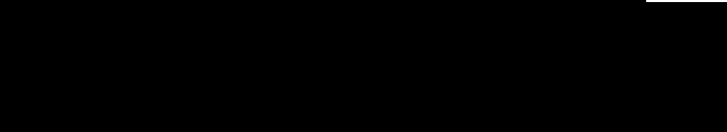
\includegraphics[width=0.9\textwidth]{pictures/primary}
\end{figure}

Natürlich kann jede der Vor- und Nachmethoden vorhanden sein oder nicht. Was zwingend vorhanden sein muss, ist eine anwendbare Primärmethode. Außerdem haben Vor- und Nachmethoden weder Wissen von, noch Einfluss auf das Ergebnis der Primärmethode. Sie eignen sich daher nur für Seiteneffekte. Dafür bieten sie der Klasse, die später erweitert wird, eine Möglichkeit, sicherzustellen, dass eine bestimmte Operation garantiert in allen Subklassen ausgeführt wird. Das kann zum Beispiel bei einer Methode zum Malen eines Bildes das Erstellen der Leinwand sein.

Zusätzlich zu Vor- und Nachmethoden gibt es noch redefinierende Methoden. Sie bestimmen selbst, ob und an welcher Stelle in ihrem Rumpf mit \texttt{call-next-method} (das CLOS-Äquivalent zu super) die nächste Methode aufgerufen werden soll. Die Aufrufreihenfolge ist wie folgt (vgl. \cite[S.103]{keene}):
\begin{itemize}
 \item CLOS ruft die spezifischste redefinierende Methode auf. Sie erhält die gleichen Parameter wie die generische Funktion bzw. Primärmethode.
 \item Falls eine redefinierende Methode \texttt{call-next-method} aufruft:
 \begin{itemize}
  \item Wenn es weitere anwendbare redefinierende Methoden gibt, wird die nächstspezifischste aufgerufen und das Ergebnis zurückgegeben.
  \item Ansonsten wird das komplette Framework aus Vor-, Primär- und Nachmethoden aufgerufen und das Ergebnis zurückgegeben.
 \end{itemize}
\end{itemize}

Es lässt sich eine Klasse Nightowl definieren, die den Rückgabewert der Primärmethode verändert:

\begin{lstlisting}
(defclass Nightowl (Trainer))

(defmethod daily-routine :around ((n Nightowl))
  (display "He slept through the whole day.\n")
  (list (call-next-method) 42))
  
> (daily-routine (make Nightowl))
\end{lstlisting}
{\routput He slept through the whole day.\\
\phantom{.}He walked out.\\
\phantom{.}He caught some Pokemon.\\
\phantom{.}He walked back home.\\
\phantom{.}(\#<void> 42)}

Da redefinierende Methoden entscheiden können, \texttt{call-next-method} nicht aufzurufen, können sie den Aufruf aller Vor-, Nach- und Primärmethoden verhindern. Eine redefinierende Methode muss auch nicht das Ergebnis der Primärmethode zurückgeben. Ein Beispiel ist die folgende Klasse Lazybum:

\begin{lstlisting}
(defclass Lazybum (Trainer))

(defmethod daily-routine :around ((l Lazybum))
  (display "And that was it.\n"))
  
> (daily-routine (make Lazybum))
\end{lstlisting}
{\routput And that was it.}

Die redefinierende Methode verhindert alle weiteren Methodenaufrufe. 

Bei mehreren Oberklassen beziehen sich die ``nächstspezifischste redefinierende Methode'' und ``alle Vor- beziehungsweise Nachmethoden'' auf den kompletten Vererbungsbaum. Es ist möglich eine Klasse Lazyowl zu definieren, die sowohl von Nightowl als auch von Lazybum erbt:

\begin{lstlisting}
(defclass Lazyowl (Nightowl Lazybum))

> (daily-routine (make Lazyowl))
\end{lstlisting}
{\routput He slept through the whole day.\\
\phantom{.}And that was it.\\
\phantom{.}(\#<void> 42)}

Ein Aufruf von \texttt{daily-routine} zeigt, dass die redefinierende Methoden beider Oberklassen aufgerufen werden. 

Im Gegensatz zu Racket sind Ergänzungsmethoden jedoch nicht kompatibel mit Methodenkombination: Sobald eine Kombination in der generischen Funktion für die Methode angegeben wird, führt der Versuch der Definition einer Ergänzungsmethode zu einem Fehler:

\begin{lstlisting}
(defgeneric daily-routine ((t Trainer))
  :combination generic-list-combination)
  
> (daily-routine (make Trainer))
\end{lstlisting}
{\routput He walked out.}

\vspace{-0.3cm}
{\rerror swindle/clos.rkt: arity mismatch; the expected number of arguments does not match the given number; expected: 2; given: 1.}

Ergänzungsmethoden sind lediglich Bestandteil der \emph{standard method combination}, also derjenigen Kombination, die ausgeführt wird, wenn keine andere Methodenkombination angegeben wurde. Sobald eine Kombination angegeben wird, ersetzt diese die \textit{standard method combination} und ein Benutzen von \texttt{:before}, \texttt{:after} und \texttt{:around} führt zu einem Fehler.

Eine Ausnahme von dieser Regel sind redefinierende Methoden, die \texttt{call-next-method} nicht aufrufen; sie sind auch in der Lage, Methodenkombination zu verhindern.

% \subsection{Ergänzungmethoden und Methodenkombination}
% Ergänzungsmethoden sind in CLOS Teil der Standard-Method-Combination (SMC), also der Methodenkombination, die ausgeführt wird, wenn wir nichts anderes angeben. Sobald wir in einer generischen Funktion eine Kombinationsart für die Methode angeben, ist es nicht mehr möglich, auch Ergänzungsmethoden für diese Methode zu definieren.
% 
% Warum ist das so?
% 
% Nehmen wir beispielsweise die \texttt{attack}-Methode aus dem Pokemonbeispiel und nehmen wir außerdem an, dass alle drei Klassen Element, Animal und Pokemon eine Around-Methode definiert haben (Abb. \ref{problem}). Die Methodenkombination sagt uns, wir müssen sowohl die Methode in Element als auch die in Animal auswerten. Pokemon besitzt jedoch eine Around-Methode, die laut SMC zuallererst ausgewertet werden müsste. Welche Regel soll zuerst befolgt werden?
% 
% \begin{figure}[h]
%  \centering
%  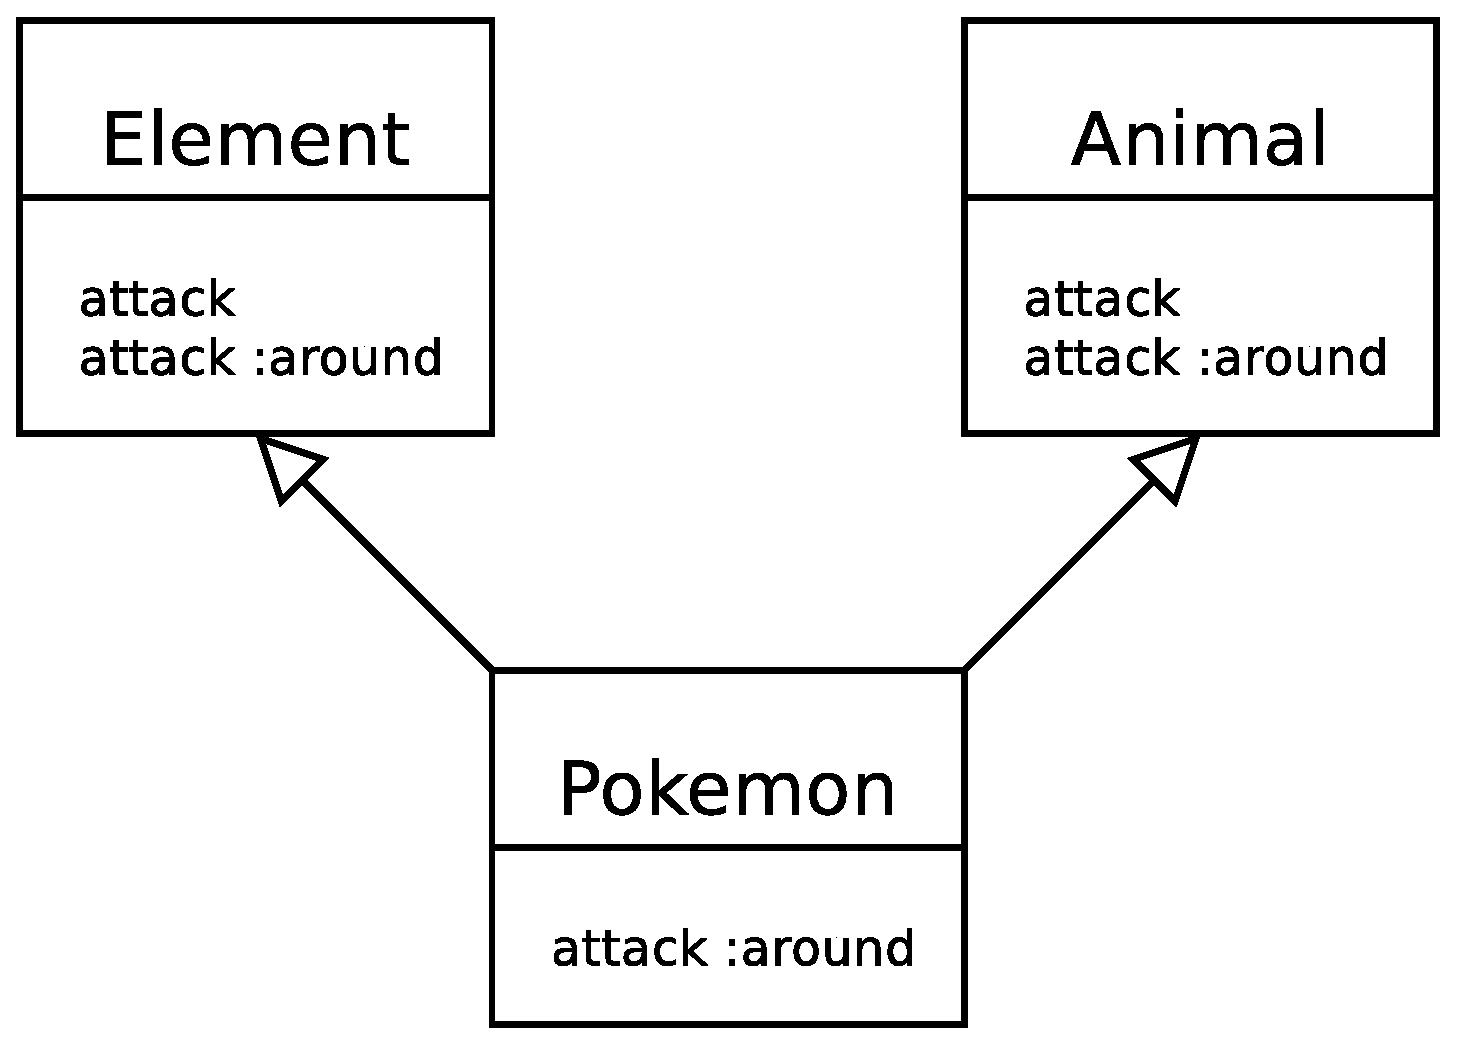
\includegraphics[scale=0.3]{pictures/problem}
%  \caption{Beispiel für Methodenkombination und Ergänzungmethoden.}
%  \label{problem}
% \end{figure}
% 
% Die naheliegende Lösung ist, den Regeln der Standard-Methodenkombination  Vorrang zu geben: wir lassen das Auswertungsschema undverändert, aber anstatt nur einer Primärmethode werten wir alle anwendbaren Primärmethoden aus und kombinieren das Ergebnis.
% 
% Zuallererst muss also die Around-Methode von Pokemon ausgewertet werden. Nehmen wir weiterhin an, die Around-Methode ruft die Methode der Superklasse auf, die spezifischste sei hier die von Element und diese ruft nicht \texttt{call-next-method} auf. Für die Listen-Kombination müssen wir jedoch die primäre Methode von Animal auswerten, die unter Umständen ohne ohne Around-Methode überhaupt keinen Sinn ergibt, zum Beispiel wenn die Around-Methode die Datei öffnet und schließt, die in der primären Methode gelesen wird.
% 
% Man müsste also alle Around-Methoden ausführen, unabhängig davon, ob \texttt{call-next-} \texttt{method} aufgerufen wurde oder nicht. Das steht jedoch in Widerspruch zu der Fähigkeit von Around-Methoden, die Auswertung anderer Methoden verhindern zu können. Die Verbindung von Methodenkombination und dem Überschreiben von Methoden scheint nicht sinnvoll. 
% 
% Vor- und Nachmethoden sind weniger problematisch, denn ihre Auswertungsreihenfolge hängt nicht von ihrem Inhalt ab. Es ist dann vermutlich

Es wurde veranschaulicht, dass ein Umgang mit Mehrfachvererbung in CLOS sehr intuitiv und einfach bereitgestellt wird.

\section{Zwischenfazit}
Das Objektsystem von Racket bietet zwar Mixins und Traits, beide sind jedoch geschickt verpackte Einfachvererbung und werden sehr kompliziert, wenn die Anzahl an Klassen steigt und gleichbenannte Methoden und Felder vorkommen. CLOS hingegen bietet einen sehr intuitiven Umgang mit Mehrfachvererbung. Es ermöglicht generische Methoden, Methodenkombination und Ergänzungsmethoden.